\documentclass{minimal}
\usepackage{graphicx,color}
\usepackage[papersize={576.00bp,432.00bp},text={576.00bp,432.00bp}]{geometry}
\begin{document}
\centering
% Title: glps_renderer figure
% Creator: GL2PS 1.3.8, (C) 1999-2012 C. Geuzaine
% For: Octave
% CreationDate: Sun Oct 25 11:51:22 2015
\setlength{\unitlength}{1pt}
\begin{picture}(0,0)
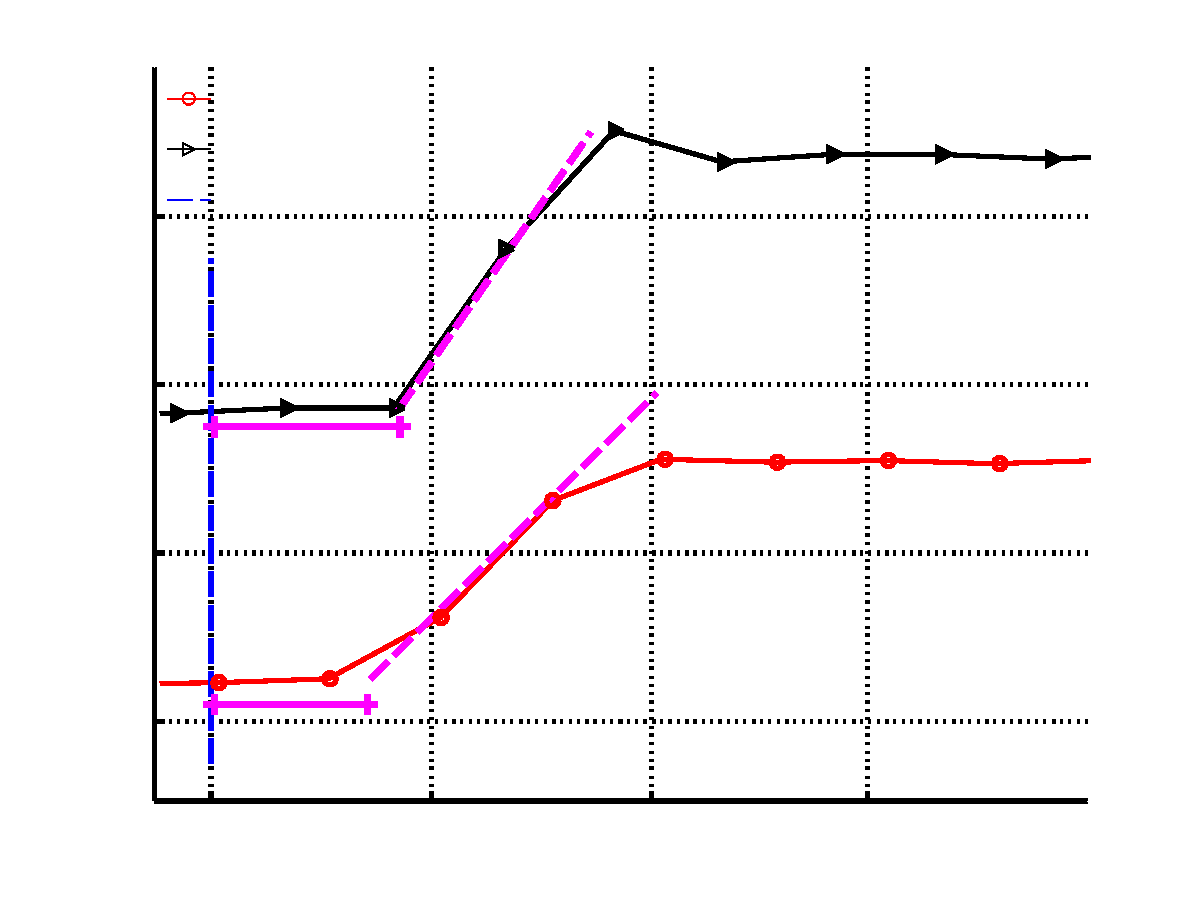
\includegraphics{ziegler-nichols-step-response-method-inc}
\end{picture}%
\begin{picture}(576,432)(0,0)
\fontsize{14}{0}
\selectfont\put(102.78,42.5189){\makebox(0,0)[t]{\textcolor[rgb]{0,0,0}{{36468.4}}}}
\fontsize{14}{0}
\selectfont\put(209.149,42.5189){\makebox(0,0)[t]{\textcolor[rgb]{0,0,0}{{36468.6}}}}
\fontsize{14}{0}
\selectfont\put(313.774,42.5189){\makebox(0,0)[t]{\textcolor[rgb]{0,0,0}{{36468.8}}}}
\fontsize{14}{0}
\selectfont\put(418.399,42.5189){\makebox(0,0)[t]{\textcolor[rgb]{0,0,0}{{36469}}}}
\fontsize{14}{0}
\selectfont\put(69.6488,85.7572){\makebox(0,0)[r]{\textcolor[rgb]{0,0,0}{{0}}}}
\fontsize{14}{0}
\selectfont\put(69.6488,166.534){\makebox(0,0)[r]{\textcolor[rgb]{0,0,0}{{20}}}}
\fontsize{14}{0}
\selectfont\put(69.6488,247.31){\makebox(0,0)[r]{\textcolor[rgb]{0,0,0}{{40}}}}
\fontsize{14}{0}
\selectfont\put(69.6488,328.086){\makebox(0,0)[r]{\textcolor[rgb]{0,0,0}{{60}}}}
\fontsize{14}{0}
\selectfont\put(299.824,21.5189){\makebox(0,0)[t]{\textcolor[rgb]{0,0,0}{{Time [sec]}}}}
\fontsize{14}{0}
\selectfont\put(52.2113,223.56){\rotatebox{90}{\makebox(0,0)[b]{\textcolor[rgb]{0,0,0}{{Power [W]}}}}}
\fontsize{14}{0}
\selectfont\put(299.824,409.6){\makebox(0,0)[b]{\textcolor[rgb]{0,0,0}{{Apparent DeadTime, L, and Steepest Slope, R, of Open-Loop Step-Response}}}}
\fontsize{14}{0}
\selectfont\put(244.024,292.415){\makebox(0,0)[l]{\textcolor[rgb]{0,0,0}{{R_{DAQ} = 189.21W/s}}}}
\fontsize{14}{0}
\selectfont\put(266.693,171.593){\makebox(0,0)[l]{\textcolor[rgb]{0,0,0}{{R_{RAPL} = 136.03W/s}}}}
\fontsize{14}{0}
\selectfont\put(109.755,206.922){\makebox(0,0)[l]{\textcolor[rgb]{0,0,0}{{L_{DAQ} = 0.17s}}}}
\fontsize{14}{0}
\selectfont\put(109.755,65.563){\makebox(0,0)[l]{\textcolor[rgb]{0,0,0}{{L_{RAPL} = 0.14s}}}}
\fontsize{14}{0}
\selectfont\put(103.676,384.686){\makebox(0,0)[l]{\textcolor[rgb]{0,0,0}{{RAPL PKG}}}}
\fontsize{14}{0}
\selectfont\put(103.676,360.344){\makebox(0,0)[l]{\textcolor[rgb]{0,0,0}{{DAQ}}}}
\fontsize{14}{0}
\selectfont\put(103.676,336.001){\makebox(0,0)[l]{\textcolor[rgb]{0,0,0}{{start of step input}}}}
\end{picture}
\end{document}
